\section{Implementasi}
\subsection{\textit{Source Code}}
Seluruh \textit{Source code} dapat dilihat dalam lampiran

\begin{verbatim}
from ucimlrepo import fetch_ucirepo 

concrete_compressive_strength = fetch_ucirepo(id=165) 
\end{verbatim}
Load seluruh dataset menggunakan \textit{package uci}

\begin{verbatim}
# Split data into train and test sets
X_train, X_test, y_train, y_test = train_test_split(
    X, y, test_size=0.2, random_state=42)

# Scale features to assist PyTorch's neural network convergence
scaler_X = StandardScaler()
scaler_y = StandardScaler()

X_train_scaled = scaler_X.fit_transform(X_train)
X_test_scaled = scaler_X.transform(X_test)

y_train_scaled = scaler_y.fit_transform(y_train)
y_test_scaled = scaler_y.transform(y_test)

# Convert arrays to PyTorch Tensors
X_train_tensor = torch.tensor(X_train_scaled, 
    dtype=torch.float32)
y_train_tensor = torch.tensor(y_train_scaled, 
    dtype=torch.float32)
X_test_tensor = torch.tensor(X_test_scaled,
    dtype=torch.float32)
y_test_tensor = torch.tensor(y_test_scaled, 
    dtype=torch.float32)
\end{verbatim}
Bagi dataset dan normalisasi 

\begin{verbatim}
grids = torch.meshgrid([torch.arange(
    num_mf) for _ in range(num_inputs)], indexing='ij')
self.rule_grid = torch.stack([g.flatten() for g in grids], 
    dim=1) # Shape: (num_rules, num_inputs)
\end{verbatim}
Inisiasi basis aturan berdasarkan jumlah fitur dan fungsi keanggotaaan

\begin{verbatim}
model = ANFIS(num_inputs=len(features), num_mf=3)
criterion = nn.MSELoss()
optimizer = optim.Adam(model.parameters(), lr=0.005)

# Training Loop
epochs = 1000
for epoch in range(epochs):
    model.train()
    optimizer.zero_grad()
    
    # Forward pass
    predictions = model(X_train_tensor)
    loss = criterion(predictions, y_train_tensor)
    
    # Backward pass and Optimization step
    loss.backward()
    optimizer.step()
    
    if (epoch + 1) % 50 == 0:
        print(f"Epoch [{epoch+1}/{epochs}] | 
            Train Loss (MSE): {loss.item():.4f}")
\end{verbatim}
Latih model

\begin{verbatim}
# Evaluation mode
model.eval()
with torch.no_grad():
    test_preds_scaled = model(X_test_tensor).numpy()

# Invert Scaling to get back metrics in real units (MPa)
test_preds = scaler_y.inverse_transform(test_preds_scaled)

# Calculate Evaluation Metrics
mae = np.mean(np.abs(test_preds - y_test))
rmse = np.sqrt(np.mean((test_preds - y_test) ** 2))
r2 = 1 - (np.sum((
    y_test - test_preds) ** 2) / 
    np.sum((y_test - np.mean(y_test)) ** 2))

print("\n--- Model Evaluation ---")
print(f"Mean Absolute Error (MAE): {mae:.2f} MPa")
print(f"Root Mean Squared Error (RMSE): {rmse:.2f} MPa")
print(f"R-squared (R²) Score: {r2:.4f}")
\end{verbatim}
Evaluasi model

\subsection{Tampilan Sistem}
Aplikasi ini di jalan kan di Jupyter Notebook dan streamlit untuk tampilan web, sebagai berikut:

\begin{figure}[H]
    \centering
    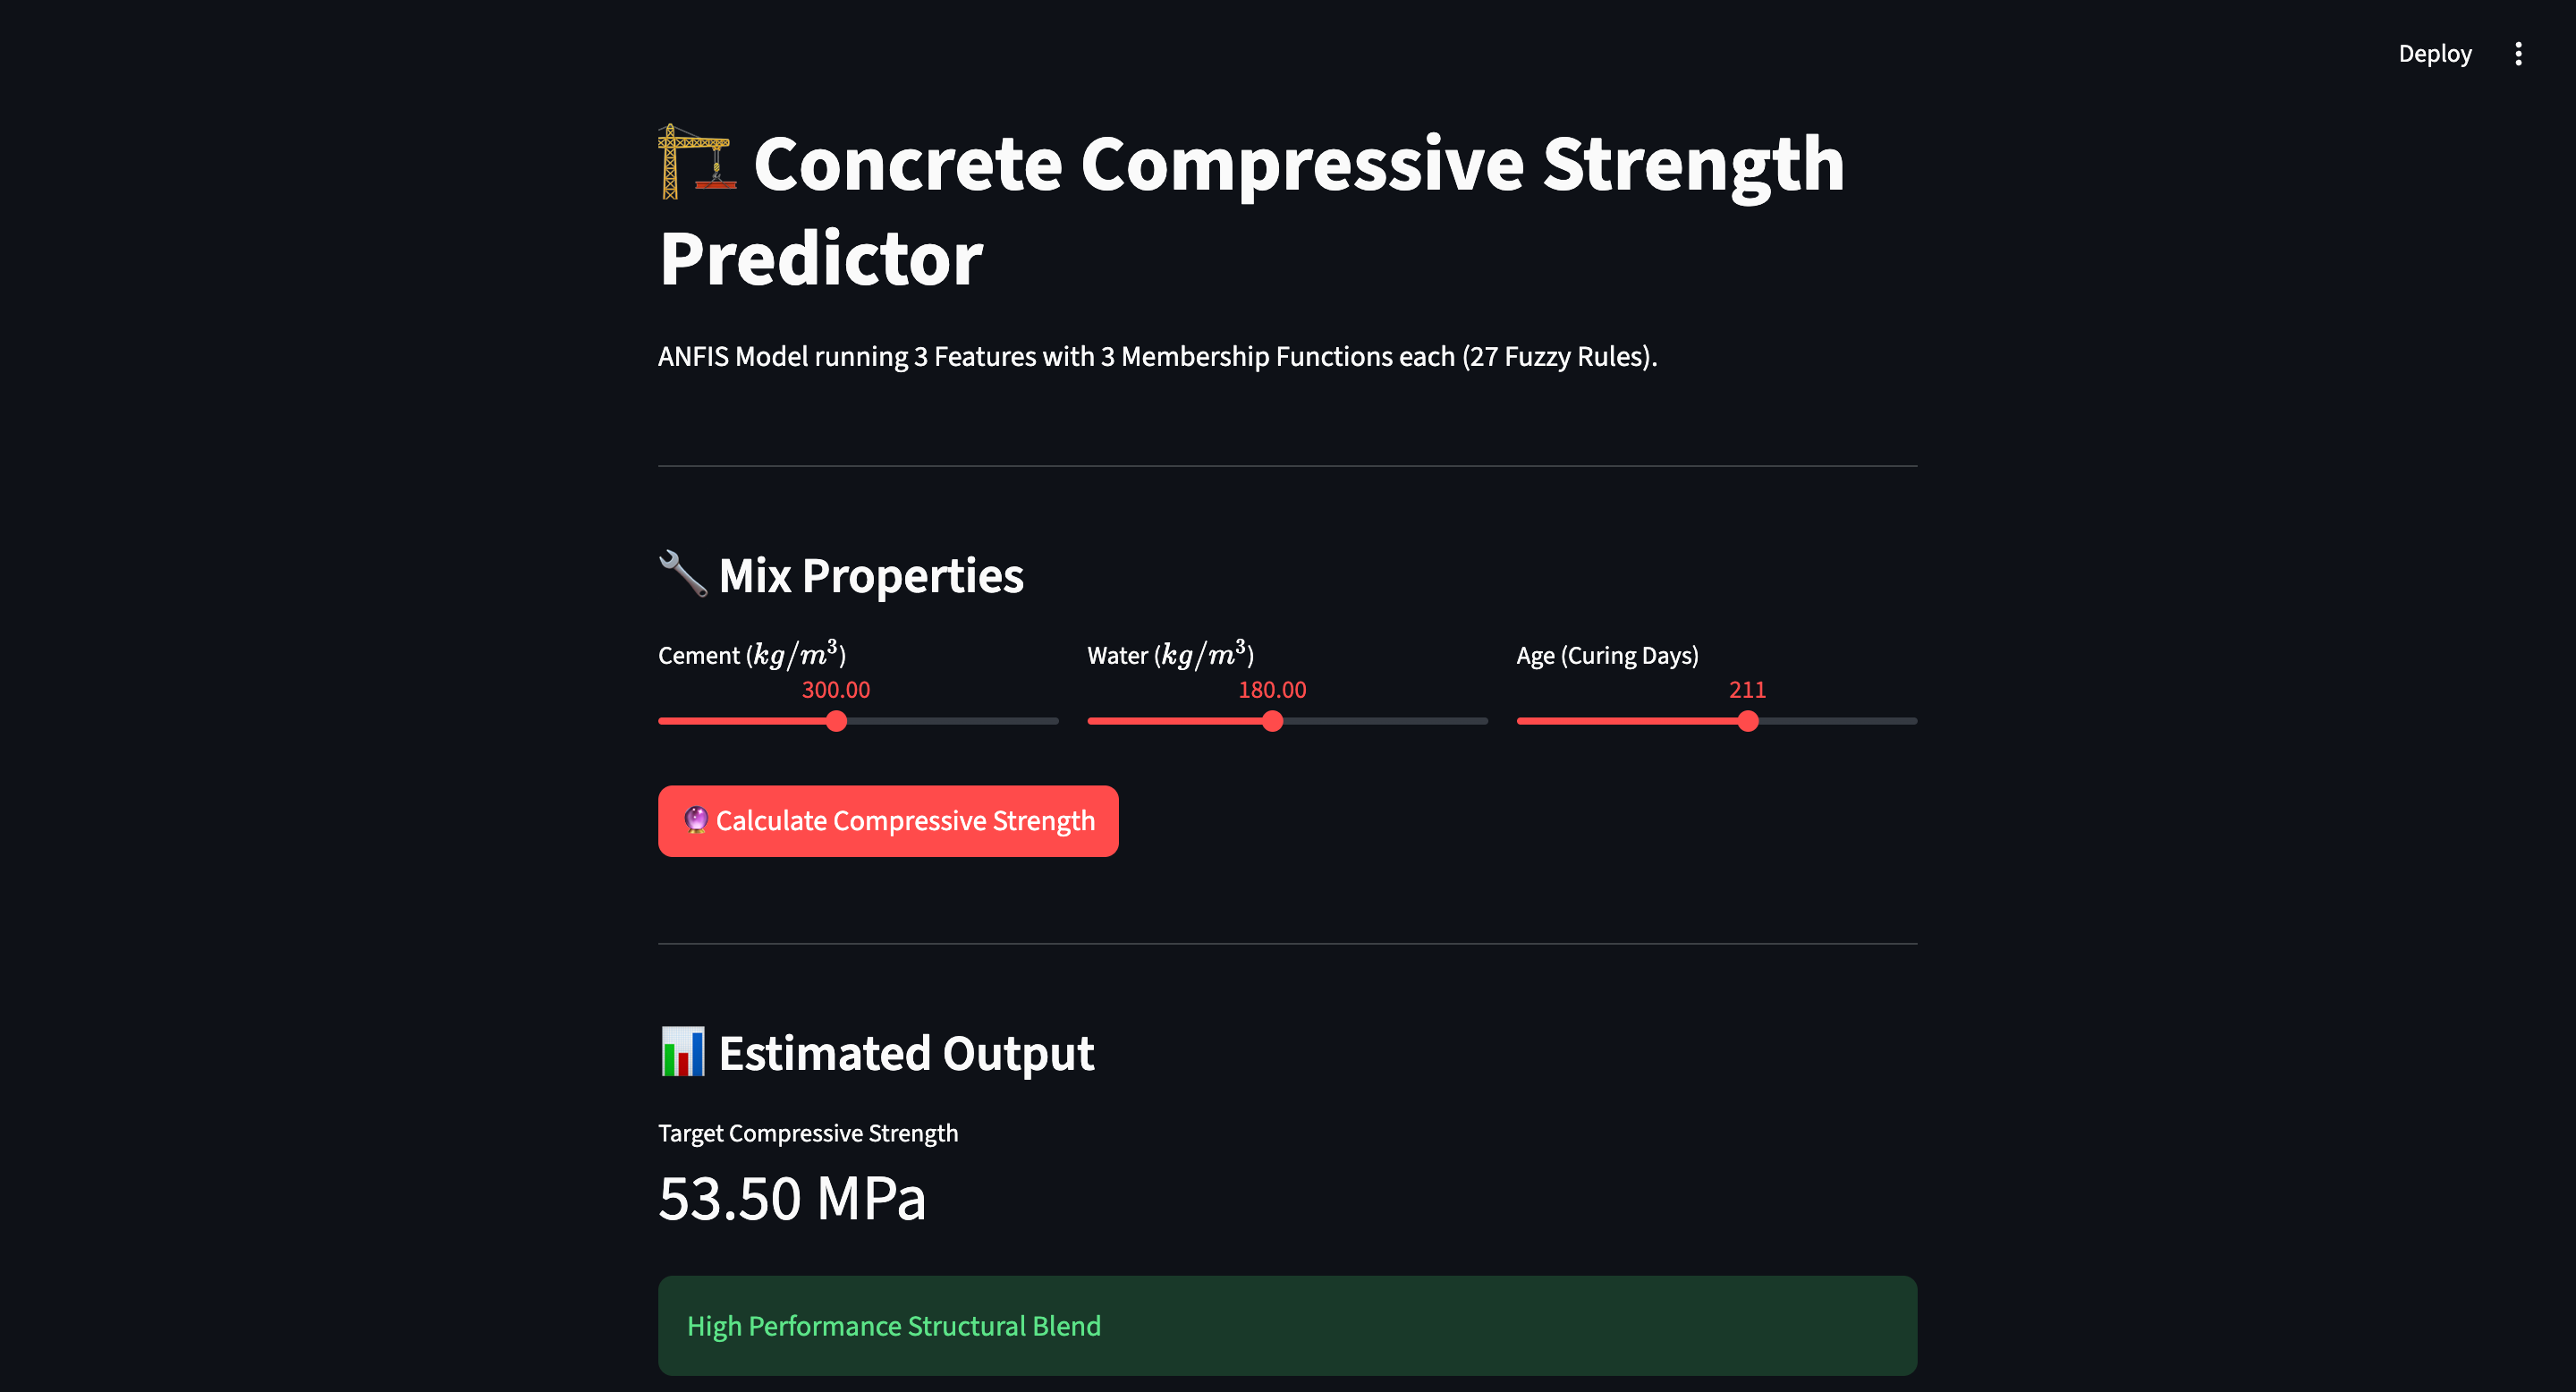
\includegraphics[width=0.8\textwidth]{streamlit.png}
    \caption{Streamlit}\label{fig:streamlit}
\end{figure}